%%%%%%%%%%%%%%%%%%%%%%%%%
\section{\applicationName} \label{projectDesign}
%%%%%%%%%%%%%%%%%%%%%%%%%
\subsection{Environment and Frameworks}
The environments selected to develop \applicationName\ are the following:
\begin{itemize}
	\item {\bf The Server--side} was written using the {\bf Java} Programming Language. The {\bf Spring Framework} was used, in particular using its most famous convention--over--configuration, called {\bf Spring Boot}. The database used to store the information about the city is {\bf MySQL}.
	\item {\bf The Client--side} was written using the {\bf Javascript} scripting language. The {\bf jQuery} library was used and, of course, {\bf HTML5} and {\bf CSS3}. As mentioned above, the 3D visualization of the city was achieved using the {\bf Cesium Framework}
\end{itemize}

\subsection{The Overall Structure}

\subsection{Server Side}
\subsubsection{Models}
\subsubsection{Parser}
\subsubsection{Cron Jobs}
\subsubsection{Controllers}
\subsection{Client Side}
\subsubsection{The first Attempt: Babylon.js}
Immediately after having gathered the essential data useful to draw the buildings of the city of Lugano, a first attempt of visualizing them was made using BabylonJS. It is a JavaScript framework for building 3D environments with HTML5 and WebGL. It allows the creation of a scene with customized lights, cameras, materials, meshes, animations, audio and actions. It also supports scene picking (i.e., an element on the scene is clickable and it is possible to interact with it).\\

In order to test the capabilities of BabylonJS, a small portion of Lugano (i.e., the part around the lake) was selected and rendered. The result can be seen in the following image:
\begin{figure}[H]
\centering
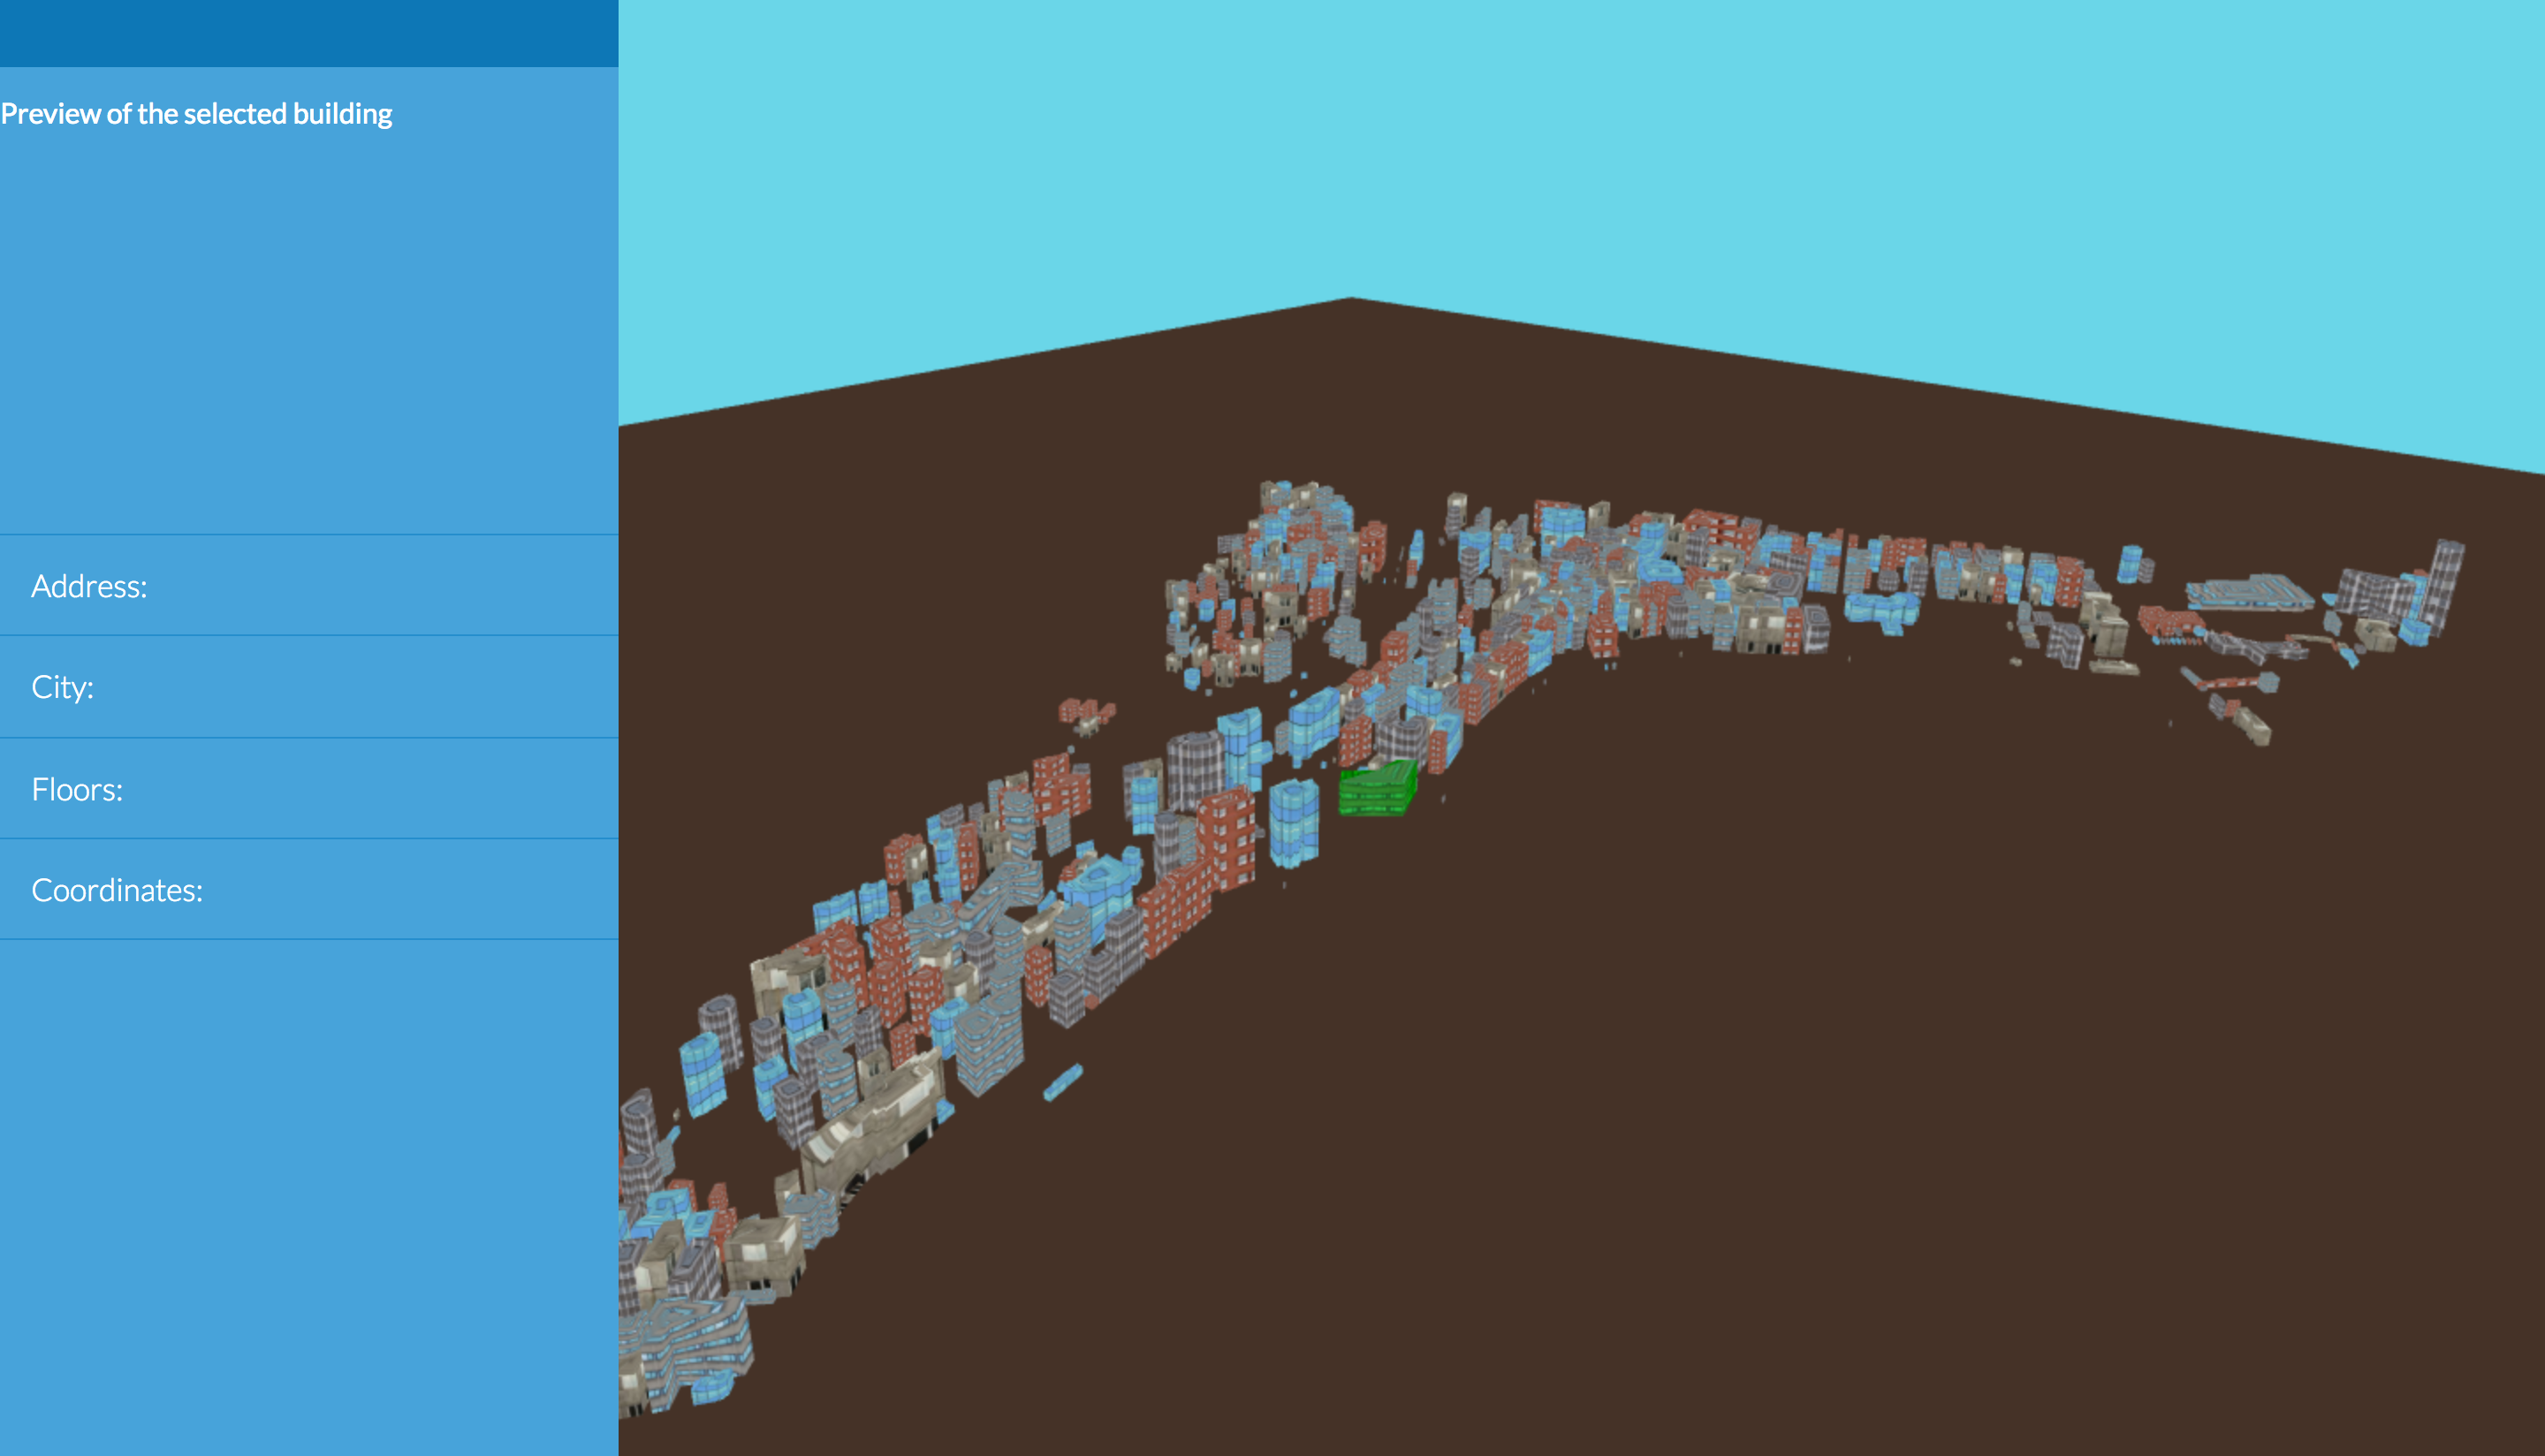
\includegraphics[width=0.8\textwidth]{chapter3/images/babylonJS}
\caption{The first attempt of city visualization using BabilonJS}
\label{fig:babilonJS}
\end{figure}
As long as the buildings showed in the scene where under the two--thousand, the browser was very fast in rendering during the loading of the page and the movement of the camera was smooth.\\
The main problems that make the idea to use BabylonJS discarded, were has been basically two:
\begin{itemize}
	\item The buildings to be rendered were far above the mentioned threshold, the rendering would take more than 30 seconds.
	\item BabylonJS provides no basis to start from: the initial scene is completely empty and, as it is possible to see in the image above, buildings lay on a plane. That represented a serious problem since the visualization of the city was planned to be shown in a way that would be as realistic as possible.
\end{itemize}
A solution to the last problem would have been using the Google Elevation API. This service, given a pair of coordinates (i.e., latitude and longitude), returns the exact altitude of that point.\\

Unfortunately, the API system of Google provides just 2,500 free requests per day. In the case of Lugano, that extends its territory for more that $25km^2$, considering one request for meter it would have been taken more than 10 days to get the entire terrain structure (for the entire city of Rome, that spans almost $46km^2$, the days taken would have been more than 20).\\

Nonetheless, this would have made the rendering slower since, in addition to the visualization of the buildings, also a rendering of the terrain (i.e., lakes, mountains and rivers) would have taken place.\\
Therefore, this lack of both Google--API--requests and good performances, lead the idea to use BabylonJS to be discarded.
\subsubsection{The final version: Cesium.js}
As stated above, the Cesium Framework was finally used to build the client--side of the application.\\
Cesium, on the contrary, provides a ready--to--use virtual globe
\subsubsection{The Side Menu and The Query Builder}
\subsubsection{Cesium Framework}